\section{Quy trình làm sạch và tiền xử lý dữ liệu}
\label{sec:data-cleaning}

Dữ liệu thô từ cả hai nguồn chứa nhiều vấn đề cần xử lý trước khi phân tích. Phần này mô tả quy trình làm sạch, được triển khai trong module \texttt{src/data/data\_cleaning.py} và orchestrate bởi \texttt{pipeline/clean\_data\_pipeline.py}.

\subsection{Xử lý chung}

\subsubsection{Loại bỏ ký tự xuống dòng}
Nhiều cột chứa ký tự \texttt{\textbackslash n} do quá trình crawl. Hàm \texttt{clean\_newlines()} thay thế tất cả \texttt{\textbackslash n} bằng dấu phẩy và loại bỏ khoảng trắng thừa cho các cột kiểu \texttt{object}.

\subsubsection{Xử lý trùng lặp}
Kiểm tra trùng lặp được thực hiện theo hai mức: (1)~trùng URL --- không có bản ghi nào trùng URL trong Chợ Tốt, (2)~trùng nội dung (title + price + brand) --- xác nhận không có trùng lặp hoàn toàn. Đối với Websosanh, không có full-row duplicate nhưng tồn tại soft duplicates (cùng cấu hình, khác shop/màu sắc).

\subsection{Xử lý dữ liệu thiếu}

Dữ liệu thiếu phân bố không đồng đều giữa các cột. \cref{tab:missing-chotot} tóm tắt tỷ lệ thiếu của nguồn Chợ Tốt.

\begin{table}[H]
    \centering
    \caption{Tỷ lệ dữ liệu thiếu các cột chính --- Chợ Tốt}
    \label{tab:missing-chotot}
    \begin{tabular}{lrr}
        \toprule
        \textbf{Cột} & \textbf{Số missing} & \textbf{Tỷ lệ (\%)} \\
        \midrule
        Card màn hình       & 1.421 & 24.2 \\
        Kích cỡ màn hình    & 1.056 & 18.0 \\
        Ổ cứng              & 470   & 8.0  \\
        Loại ổ cứng         & 854   & 14.6 \\
        RAM                 & 239   & 4.1  \\
        Bộ vi xử lý         & 237   & 4.0  \\
        Dòng máy            & 0     & 0.0  \\
        Hãng                & 0     & 0.0  \\
        \bottomrule
    \end{tabular}
\end{table}

Phân tích cho thấy missing values tuân theo mô hình \textbf{MNAR} (Missing Not At Random)\cite{rubin1976missing}: các cột spec thường thiếu cùng lúc (tương quan dương), và tỷ lệ thiếu khác nhau theo brand. Nhóm có median giá thấp hơn có xu hướng thiếu nhiều thông tin hơn.

\subsection{Chuẩn hóa và chuyển đổi kiểu dữ liệu}

\subsubsection{Giá (Price)}
\begin{itemize}[noitemsep]
    \item \textbf{Chợ Tốt}: Giá ở dạng chuỗi \texttt{"X.XXX.XXX đ"}, được parse bằng regex loại bỏ ký tự không phải số, chuyển sang numeric.
    \item \textbf{Websosanh}: Ba cột giá (\texttt{shop\_1/2/3\_price}) được chuyển về numeric bằng \texttt{pd.to\_numeric()}. Áp dụng domain filter (loại giá $<$ 3 triệu hoặc $>$ 200 triệu), sau đó tính \texttt{price\_median} từ các giá hợp lệ.
\end{itemize}

\subsubsection{RAM}
Giá trị dạng \texttt{"8 GB"} được loại bỏ ký tự chữ cái và khoảng trắng, chuyển về số nguyên (đơn vị GB). Các giá trị bất thường ($<$ 4 GB hoặc $>$ 128 GB) được kiểm tra và đánh dấu.

\subsubsection{Ổ cứng}
Hàm \texttt{clean\_storage()} xử lý nhiều trường hợp: dung lượng đơn (\texttt{"512GB"}), kết hợp (\texttt{"256GB + 1TB"}), và chuyển đổi đơn vị TB $\rightarrow$ GB (nhân 1024).

\subsubsection{Kích thước màn hình}
Extract giá trị số inch từ chuỗi text bằng regex \texttt{r"\textbackslash d+(\textbackslash.\textbackslash d+)?"}. Đối với Chợ Tốt, giá trị dạng range (\texttt{"13 -- 14.9 inch"}) được map về midpoint.

\subsubsection{CPU}
Phân loại theo ba chiều: \texttt{cpu\_brand} (Intel/AMD/Apple/Qualcomm), \texttt{cpu\_tier} (i3/i5/i7/i9, Ryzen 3/5/7/9), và \texttt{cpu\_gen} (thế hệ). Thông tin được extract từ cả cột structured và title bằng regex.

\subsubsection{GPU}
Hàm \texttt{clean\_gpu()} phân loại GPU thành các nhóm: RTX Series, GTX Series, Intel Iris Xe, Intel UHD Graphics, AMD Radeon, Intel Arc, Apple GPU, và Other GPU dựa trên keyword matching.

\subsubsection{Các cột khác}
Trọng lượng (g $\rightarrow$ kg), tốc độ CPU (GHz), độ phân giải (width $\times$ height), và kích thước vật lý (dài $\times$ rộng $\times$ dày) đều được parse từ text sang giá trị numeric.

\subsection{Kiểm tra nhất quán dữ liệu}

Các cross-check được thực hiện:
\begin{itemize}[noitemsep]
    \item \textbf{Brand vs Title}: $\sim$95\% title chứa đúng brand tương ứng trong cột Hãng.
    \item \textbf{RAM/Storage}: Giá trị extract từ title vs cột structured --- phát hiện $\sim$188 dòng conflict RAM và $\sim$96 dòng conflict storage.
    \item \textbf{Tình trạng vs Title}: $\sim$90 dòng gắn nhãn ``Mới'' nhưng title chứa keyword second-hand (``đẹp 98\%'', ``pin'', ``góp'').
    \item \textbf{Tình trạng vs Bảo hành}: Một số sản phẩm ``Mới'' nhưng ``Hết bảo hành''.
\end{itemize}

\begin{figure}[H]
    \centering
    % FILL-IN: [USER] Thêm biểu đồ missing value heatmap
    % Nguồn: notebook 01a_chotot_inspection.ipynb, cell [25] — msno.heatmap()
    % \includegraphics[width=0.7\textwidth]{images/missing-heatmap.png}
    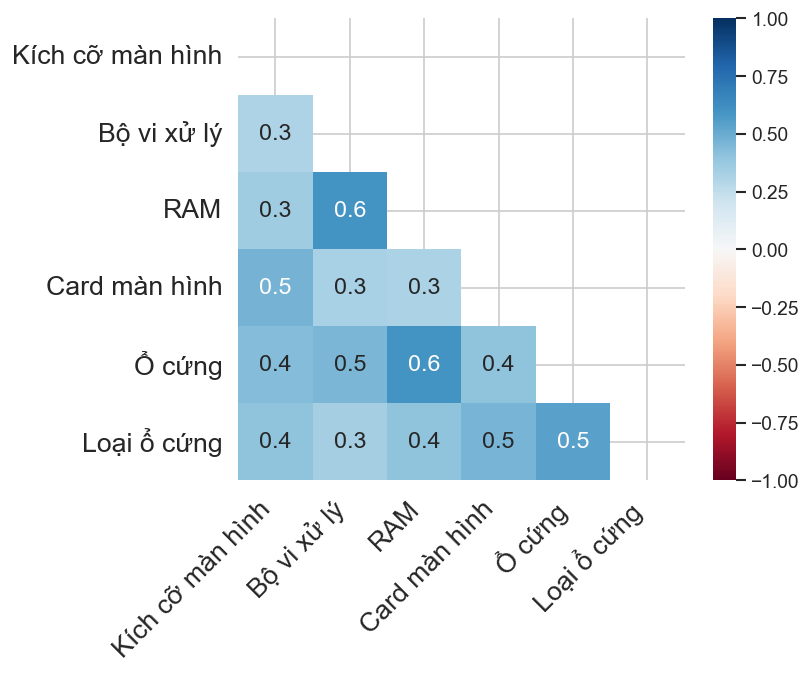
\includegraphics[width=0.7\textwidth]{images/chotot_img_04.png}
    \caption{Heatmap tương quan giữa các cột thiếu dữ liệu trong dataset Chợ Tốt. Giá trị dương (màu sáng) cho thấy các cột spec có xu hướng thiếu cùng lúc, xác nhận mô hình MNAR.}
    \label{fig:missing-heatmap}
\end{figure}
